\section{Nombres de Fine, relations de similarité et permutation}
\subsection{Relations de similarité}
\begin{frame}{Quelques définitions}
    \begin{block}{Définition 1}
        Une relation de similarité $\mathcal{R}$ sur [n] est une relation binaire, réflexive et symétrique
		vérifiant la propriété suivante:
		$$\forall x, y, z \in [n], \left((x<y\leq z \text{ et } x\mathcal{R}z) \implies
			(x\mathcal{R}y \text{ et } y\mathcal{R}z)\right) $$
        On note par $RS_{n}$ l'ensemble de tels relations.
    \end{block}
    \begin{block}{Définition 2}
        Soit $i \in [n]$. On dit que $i$ est un point isolé de $\mathcal{R}$ si \\
		$$\forall j \in [n], (i\mathcal{R} j\implies i=j) $$
    \end{block}
    \begin{block}{}
        On note par Sim$_{n}$ l'ensemble des mots $r=r_{1} r_{2}\cdots r_{n}$, avec les $r_{i}\in\mathbb{N}$, tels que
    $\forall i\leq n, 0\leq r_{i} \leq i-1 \text{ et }  r_{i+1}\leq r_{i}+1$ avec la convention $r_{n+1}=0$
    \end{block}
\end{frame}

\begin{frame}{Conditions nécessaire et suffisante}
    \transfade
    \begin{block}<1->{Proposition 1}
        La transformation $\Phi: $\rm{RS}$_{n} \rightarrow $\rm{Sim}$_{n}$, $\mathcal{R} \rightarrow r = r_{1}r_{2}\cdots r_{n}$ \textit{ où, pour }$1\leq i \leq n$ , $r_{i}$ \textit{est égale au nombre d'entiers} $j$ \textit{tels que} $j<i$ \textit{et} $j\mathcal{R}i$, \textit{est une application bijective.}\\ De plus, 
        $|$Sim$_{n}(k)|:=\{r \in $ Sim$_{n}; \#\{i; r_{i}=r_{i+1}=0\}=k\} = \#$RS$_{n}(k)$ 
         $\mathcal{R}$
    \end{block}
    \begin{block}<2->{Proposition 2}
        Soit la transformation $\varphi$ : $ $\rm{Dyck}$(n) \longrightarrow $\rm{Sim}$_n$, $p=p_{1}p_{2}\cdots p_{2n} \longrightarrow r=r_{1}r_{2}\cdots r_{n}$ \textit{définie comme suit}:\\
        \textit{Soit} \rm{Mont}$(p)=\{i_{1}, i_{2}, \cdots, i_{n}\}$ \textit{l'ensemble des entiers} $i$ tels que $p_{i}=m$. \textit{Alors pour tout }$1\leq j \leq n$, $r_{j} = \gamma_{i_{j}-1}$ \textit{où} $\gamma_{i-1}$ \textit{est le niveau du} $i$\textit{-ième pas de p.}
        \textit{Alors} $\varphi$ \textit{est une application bijective}.\\
        \textit{De plus}, $|$\rm{Sim}$_{n}(k)| = \# \{p \in $\rm{Dyck}$(n); |\{i \in $\rm{Mont}$(p); \gamma_{i-1}=0 \text{ et } p_{i+1}=d\}|=k\}$
    \end{block}
\end{frame}

\begin{frame}{Les relations de similarité non-singulière}
    On en déduit les résultats suivants en utilisant les deux bijections précédentes et la bijection $\theta$ sur les chemins de Fine:
    \begin{itemize}
        \item $\{p \in $\rm{Dyck}$(n); |\{i \in $\rm{Mont}$(p); \gamma_{i-1}=0 \text{ et } p_{i+1}=d\}|=0\}$ = $\overline{\rm{Dyck}}(n)$
        \item $|$RS$_{n}(0)|=F_{n}$ où $F_{n}$ est la cardinalité de $|\mathcal{F}_n|$
    \end{itemize}
\end{frame}


\subsection{Autres interprétations des $F_{n}$}
\begin{frame}{Les permutations évitant le motif 123}
    \transfade
    \begin{block}{Proposition 1}
        Soit $\Theta$ la transformation $S_{n}(123) \longrightarrow$ \rm{Dyck}$(n)$, $\pi \longrightarrow p$ \textit{définie par}:\\
        \textit{soit} $w_{1}u_{1}w_{2}u_2 \cdots w_{s}u_{s}$ \textit{la ssd-décomposition de $\pi$ et on définit $\Theta(\pi):=p=m_{1}d_{1}m_{2}d_{2}\cdots m_{s}d_{s}$ où $m_{i}$ (resp $d_{i}$) est un mot formé par la seule lettre $m$ (resp $d$) tel que $|m_{i}| = |w_{i}|+1$ et $|d_{i}| = u_{i}-u_{i+1}$ avec la convention $u_{s+1}=0$.}\\
        \textit{Alors $\Theta$ est bijective.}\\
        \textit{De plus, $\#D(\pi) = \#\{i\in$ \rm{Mont}$(p)$$;\gamma_{i-1}=0, p_{i+1}=d\}$} où $D(\pi):=\{i; \pi_{n-i+1}=i\}$
    \end{block}
    \pause
    \begin{block}{Corollaire 1}
        On a $\forall n \geq 0, s_{n}^{k}(321)=\#$\rm{RS}$_{n}(k)$
    \end{block}
    \pause
    \begin{block}{Corollaire 2}
        On a $F_{n} = s_{n}^{0}(321)$.
    \end{block}
\end{frame}

\begin{frame}{Interprétations combinatoire des $F_{n}$}
    \transfade
    \begin{block}{Proposition 1}
        Pour tout $\mu \in \{123, 132\}$, on a $F_{2n}=\#\{ \sigma \in S_{2n}(\mu); \sigma(1) \text{ impair }\}$ et $F_{2n+1} = \#\{\sigma\in S_{2n+1}(\mu); \sigma(1) \text{ pair }\}$
    \end{block}
    \pause
    \begin{block}{Proposition 2}
        Pour tout $n\geq 1$, on a $F_{n} = \#\{\pi \in S_{n}(\mu); \text{Fix}(\pi)\bigcap [n-1]\neq \emptyset\}$
    \end{block}
\end{frame}

\begin{frame}{Mots de Catalan}
    \begin{block}{Définition}
        A un décalage d'indice, un chemin de Dyck de longueur $2n$ est représenté par un mot $c_{1}c_{2}
        \cdots c_{n}$ tel que $1 \leq c_{1} \leq c_{2} \leq \cdots \leq c_{n}$ où \\ $c_{i} \leq i$ pour
        tout $i$. Un tel mot est appelé mot de Catalan de longueur $n$. On note par Cat$(n)$ l'ensemble des mots de Catalan  de longueur $n$.
    \end{block}
    \begin{figure}[h!]
        \centering
        \begin{subfigure}[b]{0.38\textwidth}
            \centering
            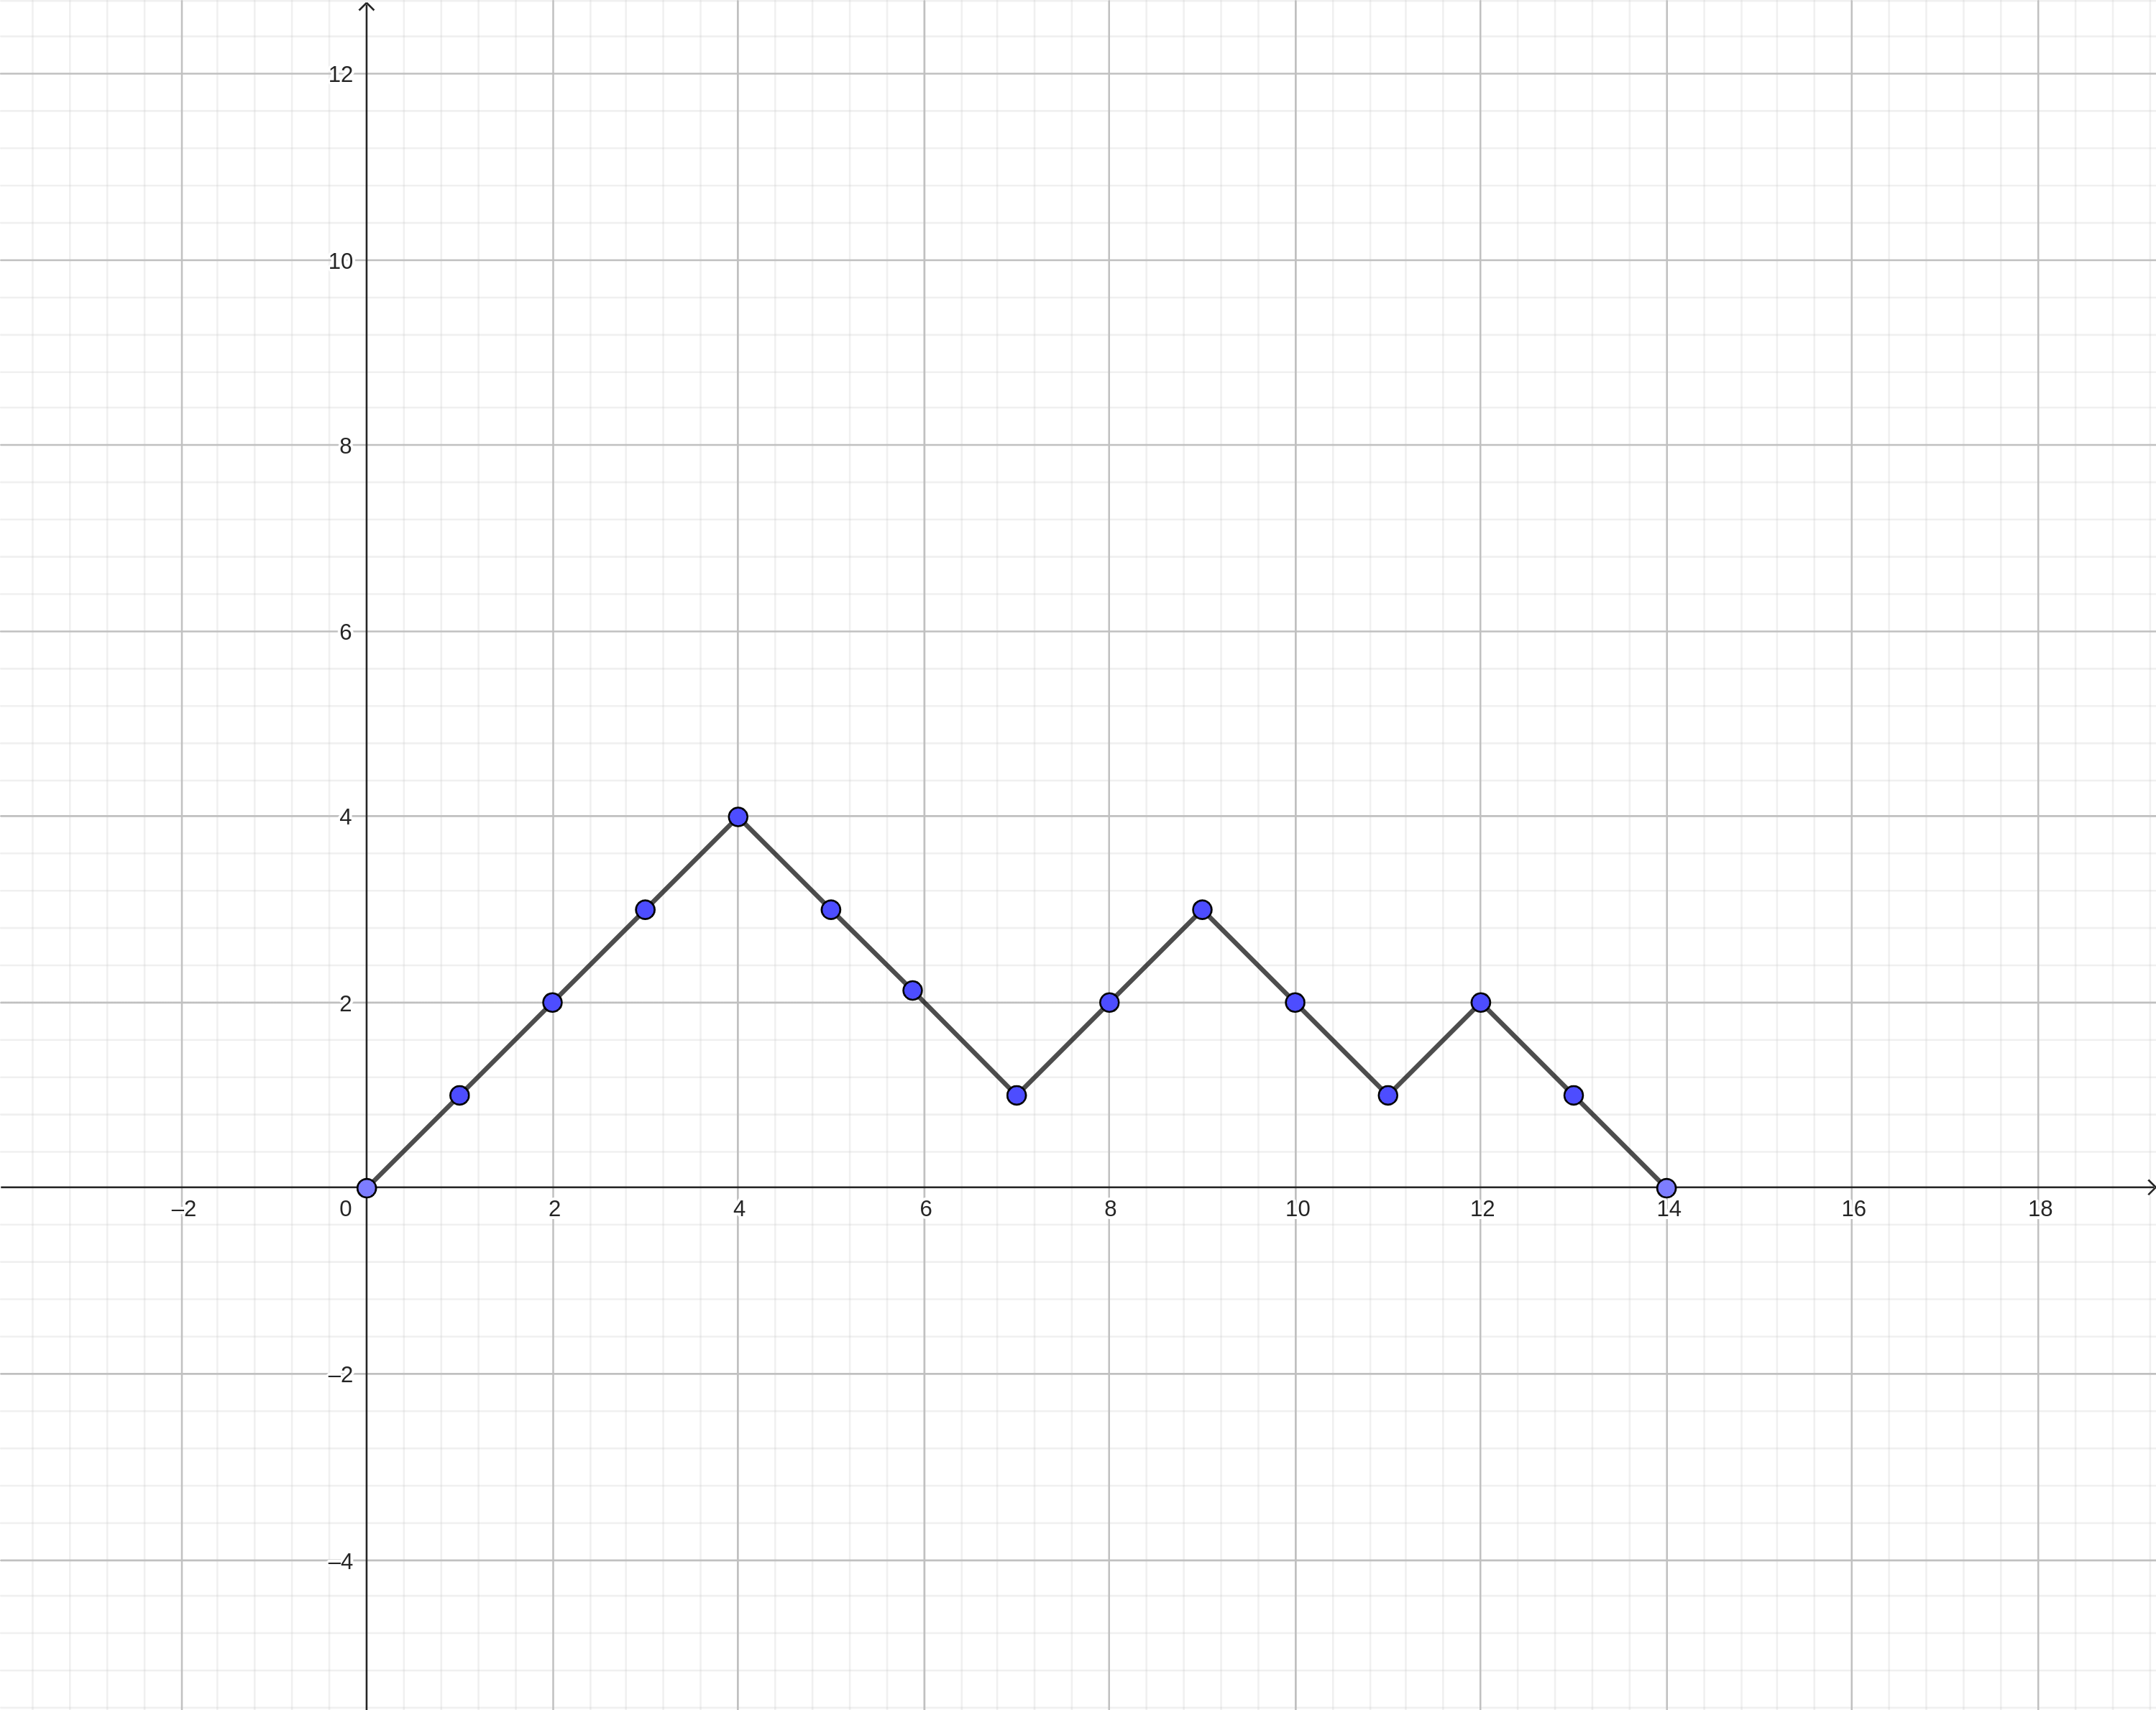
\includegraphics[width=\textwidth]{./images/dyck path.png}
            \caption{Chemin de Dyck}
        \end{subfigure}
        \hspace{1cm}
        \begin{subfigure}[b]{0.38\textwidth}
            \centering
            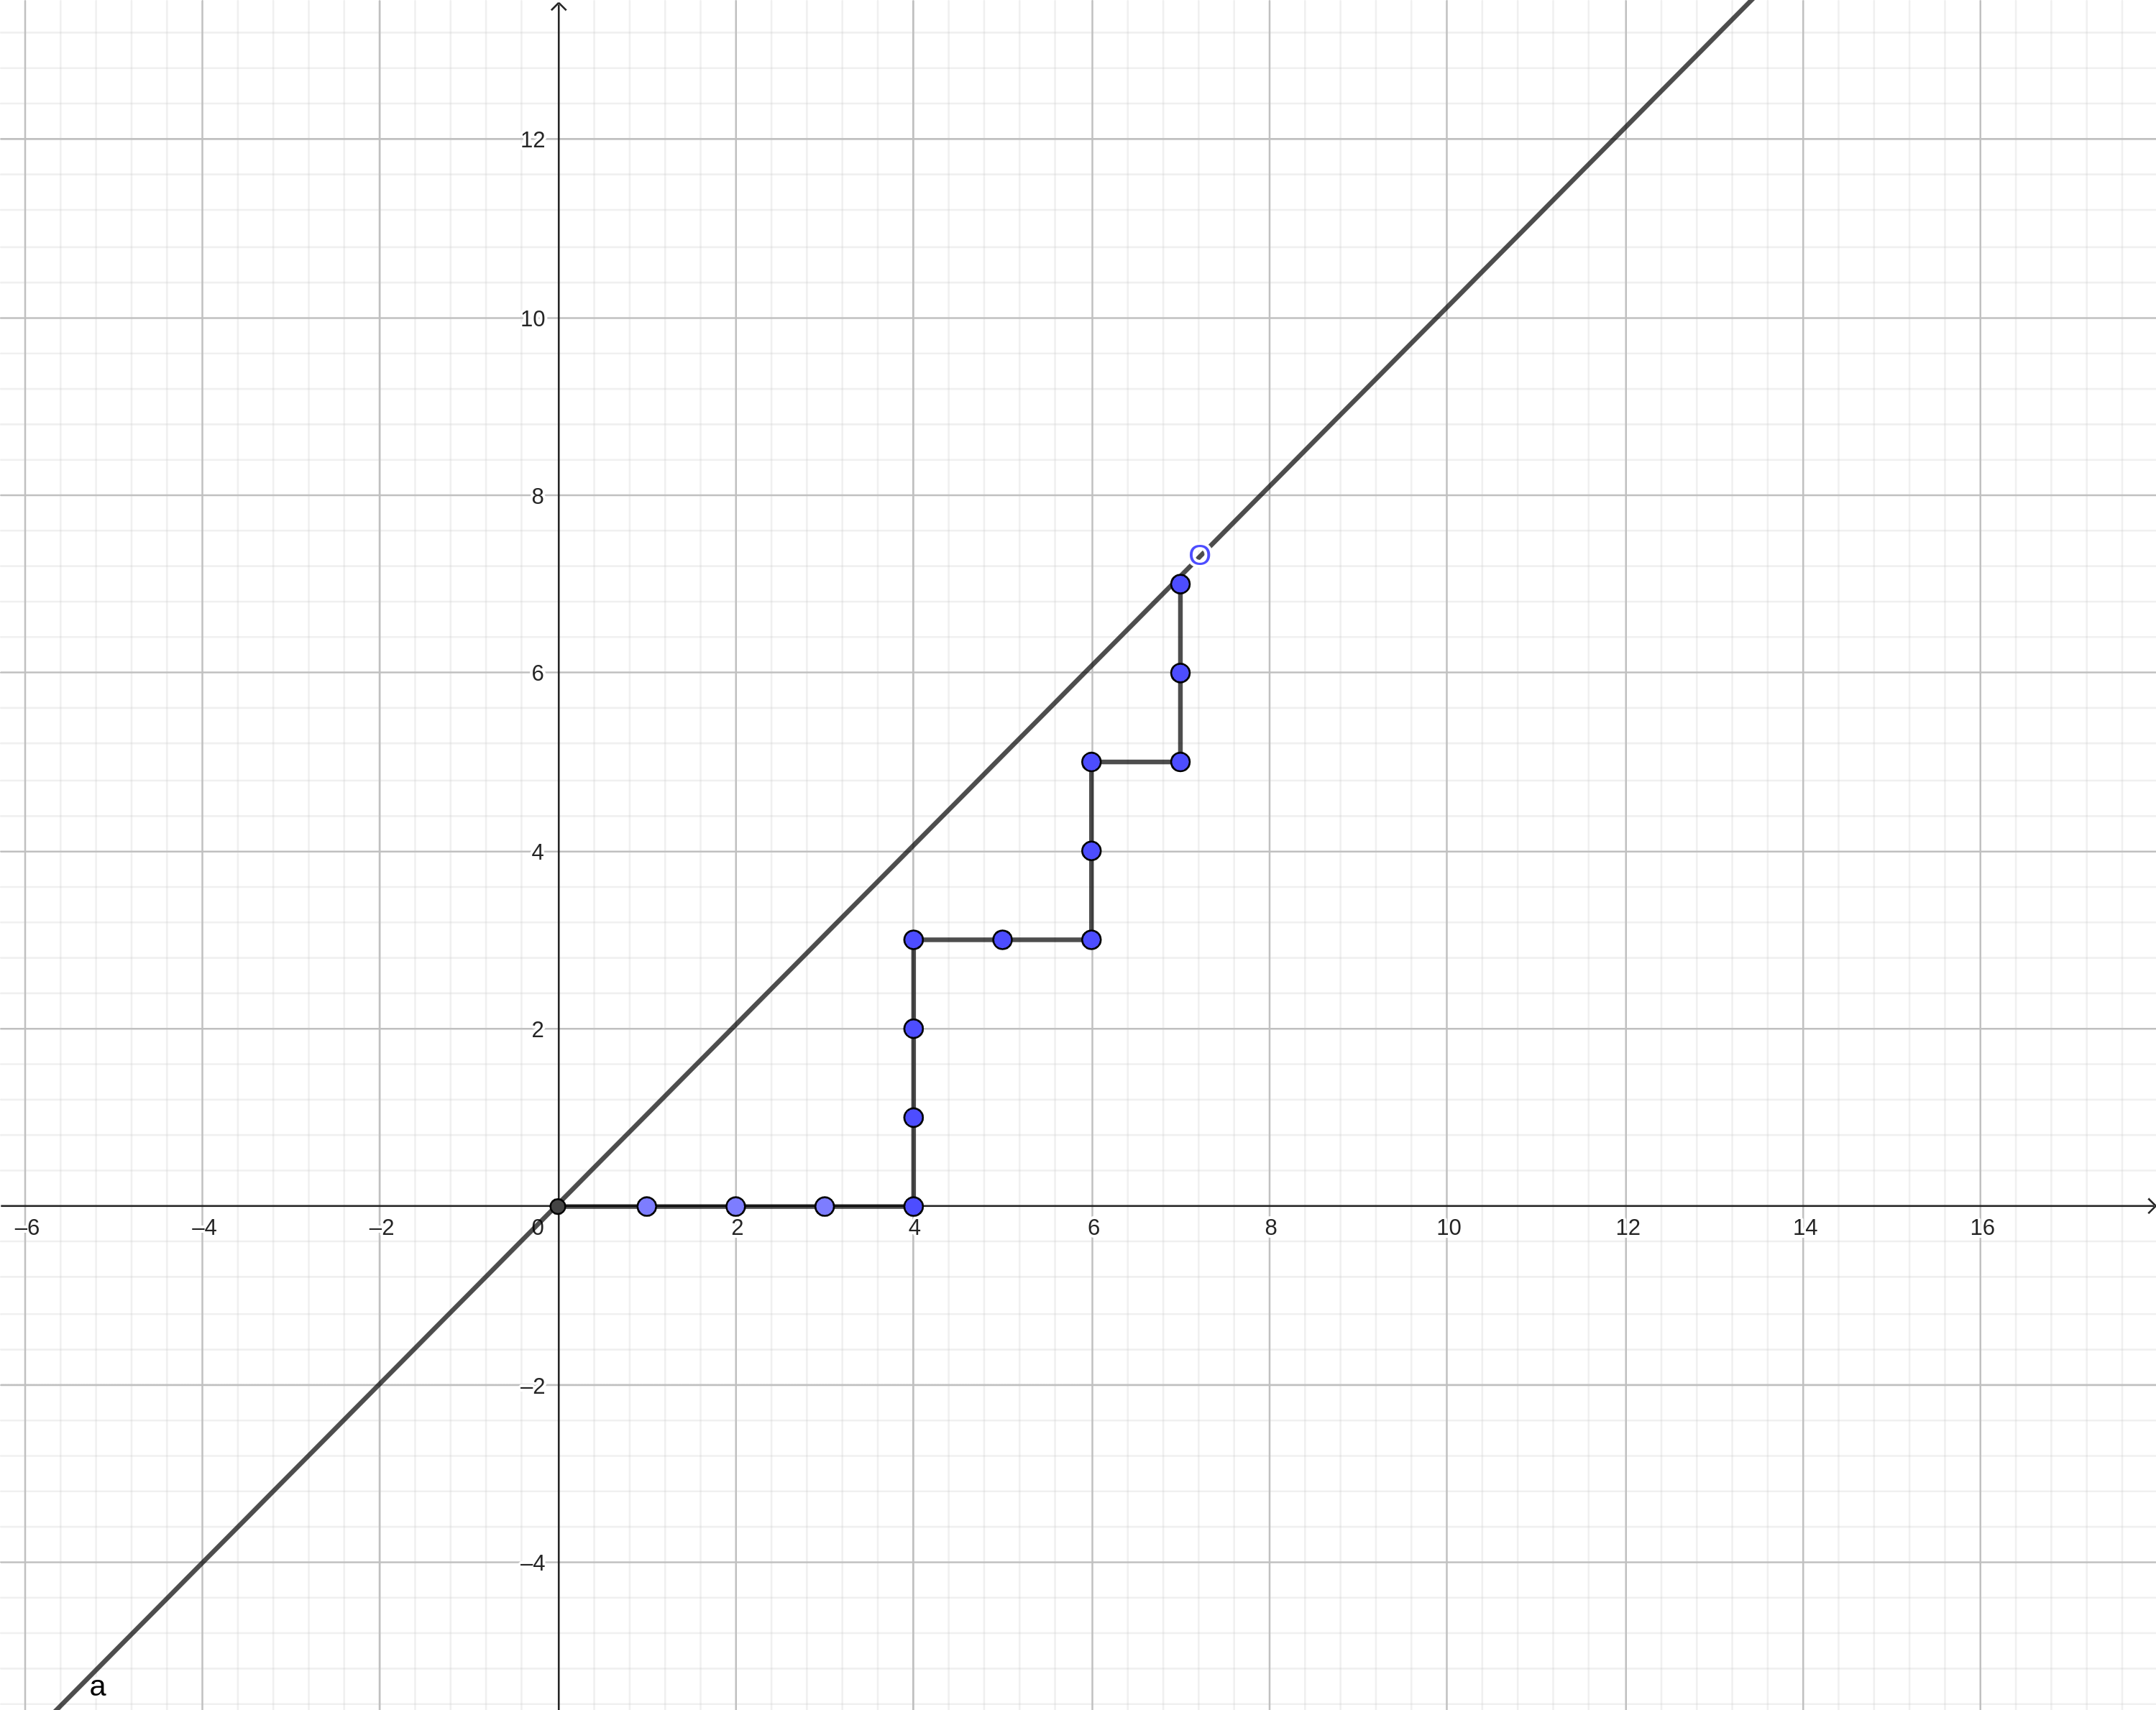
\includegraphics[width=\textwidth]{./images/transformed-dyck path.png}
            \caption{Transformé du chemin de Dyck}
        \end{subfigure}
        \caption{Nouveau chemin de Dyck}
        \label{fig:DyckPath}
    \end{figure}
    
\end{frame}

\begin{frame}[t]{Quelques résultats}
    On pose $A_{n}(x)=\sum\limits_{\pi \in S_{n}(321)}x^{fix(\pi)}$
    \transfade
    \begin{itemize}
        \item $A_{n}(x)=\sum\limits_{c \in Cat(n)}x^{\#D(c)}$ où $D(c)=\{i; c_{i}=i \text{ et }c_{i+1}=i+1\}$
        \pause
        \item $s_{n}^{k}(321)=\#\{c\in Cat(n); |D(c)|=k\}$
        \pause
        \item $1+\sum\limits_{n\geq 1}A_{n}(x)z^{n}=\cfrac{1-x+C(z)}{2-x+z(x-1)^{2}}$
        \pause
        \item $A_{n}(x) = (x-1)A_{n-1}(x) + \sum\limits_{i=1}^{n}C_{i-1}A_{n-i}(x)$n
        \pause
        \item $A_{n}(x)=(x-1)^{n}+\sum\limits_{i=0}^{n-1}(x-1)^{i}\sum\limits_{i=1}^{n-i}C_{j-1}A_{n-i-j}(x)=\sum\limits_{k=0}^{n}b(n,k)(x-1)^{k}$
        \pause
        \item $[x^{k}]A_{n}(x)=\sum\limits_{j=k}^{n}\binom{k}{j}b(n,k)(-1)^{j-k}$
        \pause
        \item $\forall n\geq 1 \text{ et }\forall k\leq n, b(n, k) = b(m, k+1) + b(n-1, k-1)$

    \end{itemize}
\end{frame}

\begin{frame}
    \transfade
    \begin{block}{Définition}
        Le triangle de Catalan est défini comme suit:
        $$
            \begin{cases}
                c_{n, 0} & = 1, \forall n\geq 0                                 \\
                c_{n, k} & = 0, \text{ si } n<k \text{ ou } n<0 \text{ ou } k<0 \\
                c_{n, k} & = c_{n-1, k} + c_{n, k-1}, \forall k, n \geq 1
            \end{cases}
        $$
    \end{block}
    \pause
    \begin{block}{Lemme}
        Soit $s_{n, k} (p)$ le nombre de permutations $\sigma$ dans $S_{n}(p)$ vérifiant $\sigma(1)=k$. On a pour tout $n, k \geq 1$, $s_{n,k}(123) = s_{n,k}(132) = s_{n, n-k+1}(321) = c_{n-1, k-1}$\\ (Voir \cite{Desantis})
    \end{block}
\end{frame}

\begin{frame}
    A partir des deux tableaux suivants, on déduit les deux propositions ci-après.\\
Le tableau $(b(n, k))$ est
$$
	\begin{matrix}
		1  &                  \\
		1  & 1  &             \\
		2  & 2  & 1 &         \\
		5  & 5  & 3 & 1 &     \\
		14 & 14 & 9 & 4 & 1 & \\
	\end{matrix}
$$
et le tableau $(c_{n, k})$ est
$$
	\begin{matrix}
		1 &                   \\
		1 & 1 &               \\
		1 & 2 & 2 &           \\
		1 & 3 & 5 & 5  &      \\
		1 & 4 & 9 & 14 & 14 & \\
	\end{matrix}
$$
\end{frame}
\begin{frame}
    \transfade
    \begin{block}{Proposition 1}
        $\forall n\geq k, b(n,k)=c_{n, n-k}$
    \end{block}
    \pause
    \begin{block}{Proposition 2}
        On a $F_{n} = \sum\limits_{k=0}^{\lfloor \frac{n}{2} \rfloor}c_{n-1, n-2k}$
    \end{block}
\end{frame}

\begin{frame}
    \transfade
    On conclut que $F_{2n}=\#\{ \sigma \in S_{2n}(\mu); \sigma(1) \text{ impair }\}$ et $F_{2n+1} = \#\{\sigma\in S_{2n+1}(\mu); \sigma(1) \text{ pair }\}$ pour $\mu=321$. \\
    \vspace{5pt} On note $\mathcal{E}_{n,r}$ l'ensemble des bijections $\pi$ de $[n]$ vers $\{r+1, \cdots, r+n\}$ telles que
    st$(\pi) \in S_{n}(132)$ et considérons la fonction génératrice $E_{n,r}(x) = \underset{\pi \in \mathcal{E}_{n,r}}{\sum}x^{\text{fix}(\pi)}$
    où l'on convient $E_{0,r}(x)=1$
    \begin{block}{Proposition}
        On a $E_{n, r}(x)=A_{n}(x) + (1-x)\sum\limits_{i=0}^{r}C_{i-1}A_{n-i}(x)$
    \end{block}
    \pause
    \begin{block}{Corollaire}
        On a $A_{n}(x) = \sum\limits_{\pi \in S_{n}(132)}x^{fix(\pi)}$
    \end{block}
\end{frame}
\begin{frame}
\end{frame}